
\begin{figure*}[t]
\captionsetup{font=small}
\begin{center}
\begin{tabular}{c@{~~~~~}c}
Verification ROC & Identification DET \\
{\scriptsize (higher is better)} & {\scriptsize (lower is better)} \\ [0.1cm]
%
%
%
%
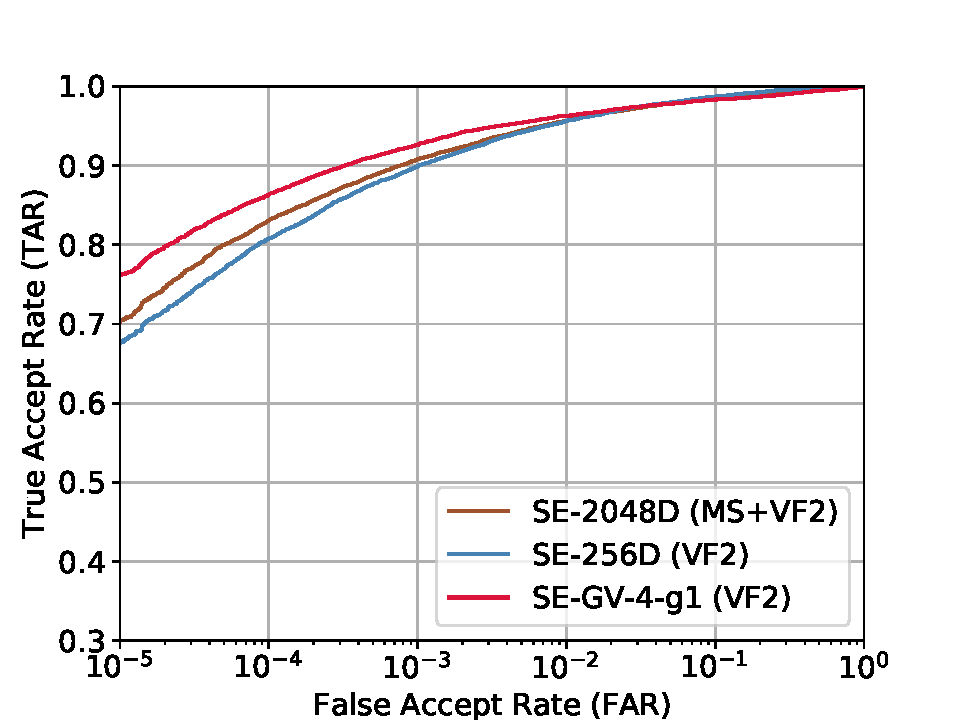
\includegraphics[align=c,width=44mm,clip,trim=0 0 0 1cm]{images/roc_ijbb} &
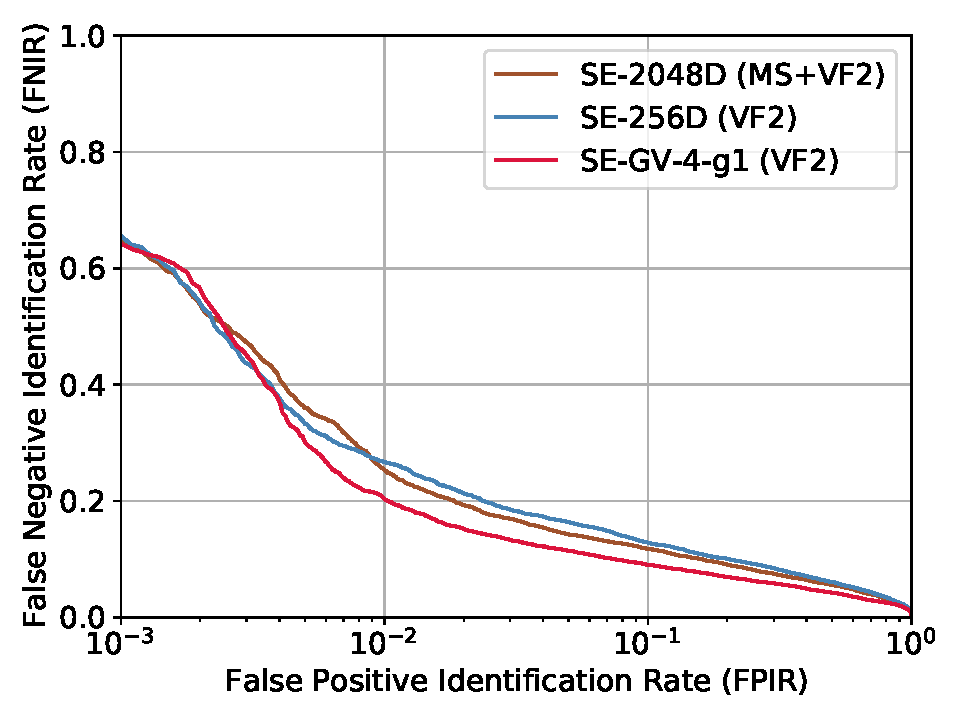
\includegraphics[align=c,width=42mm,clip,trim=0 0.5cm 0 0]{images/1N_DET_ijbb}
\end{tabular}
\end{center}
\vspace{-2mm}
\caption{{\bf Results on the IJB-B dataset.} 
%
%
Our \emph{SE-GV-4-g1} network which produces 128-D templates,
beats the best baseline (\emph{SE} with 256-D templates)}
and the state-of-the-art trained on a much larger dataset
(\emph{SE} with 2048-D templates) trained on VGGFace2 and MS-Celeb-1M).
\label{fig:ijb}
\vspace{-4mm}
\end{figure*}



